\documentclass{sigchi}

% Arabic page numbers for submission. 
% Remove this line to eliminate page numbers for the camera ready copy
\pagenumbering{arabic}


% Load basic packages
\usepackage{balance}  % to better equalize the last page
\usepackage{graphics} % for EPS, load graphicx instead
\usepackage{times}    % comment if you want LaTeX's default font
\usepackage{url}      % llt: nicely formatted URLs


% llt: Define a global style for URLs, rather that the default one
\makeatletter
\def\url@leostyle{%
  \@ifundefined{selectfont}{\def\UrlFont{\sf}}{\def\UrlFont{\small\bf\ttfamily}}}
\makeatother
\urlstyle{leo}


% To make various LaTeX processors do the right thing with page size.
\def\pprw{8.5in}
\def\pprh{11in}
\special{papersize=\pprw,\pprh}
\setlength{\paperwidth}{\pprw}
\setlength{\paperheight}{\pprh}
\setlength{\pdfpagewidth}{\pprw}
\setlength{\pdfpageheight}{\pprh}

% Make sure hyperref comes last of your loaded packages, 
% to give it a fighting chance of not being over-written, 
% since its job is to redefine many LaTeX commands.
\usepackage[pdftex]{hyperref}
\hypersetup{
pdftitle={SIGCHI Conference Proceedings Format},
pdfauthor={LaTeX},
pdfkeywords={SIGCHI, proceedings, archival format},
bookmarksnumbered,
pdfstartview={FitH},
colorlinks,
citecolor=black,
filecolor=black,
linkcolor=black,
urlcolor=black,
breaklinks=true,
}

% create a shortcut to typeset table headings
\newcommand\tabhead[1]{\small\textbf{#1}}

\newcommand{\croder}{\textbf{Croder }}
\newcommand{\IDE}{\textbf{IDE }}
\newcommand{\eclipse}{\textbf{Eclipse }}


\title{Croder: Bringing the Knowledge of the Crowds into the IDE}
\author{Semih Okur \and Mihai Codoban \and Caius Brindescu \and Kyungho Lee \and Shuo Yuan}
\numberofauthors{5}
\author{
  \alignauthor Semih Okur\\
    \affaddr{University of Illinois at Urbana-Champaign}\\
    \affaddr{Urbana, IL}\\
    \email{okur2@illinois.edu}
  \alignauthor Mihai Codoban\\
    \affaddr{University of Illinois at Urbana-Champaign}\\
    \affaddr{Urbana, IL}\\
    \email{codo@illinois.edu}
  \alignauthor Caius Brindescu\\
    \affaddr{University of Illinois at Urbana-Champaign}\\
    \affaddr{Urbana, IL}\\
    \email{brind@illinois.edu}
   \alignauthor Kyungho Lee\\
    \affaddr{University of Illinois at Urbana-Champaign}\\
    \affaddr{Urbana, IL}\\
    \email{klee141@illinois.edu}
  \alignauthor Shuo Yuan\\
    \affaddr{University of Illinois at Urbana-Champaign}\\
    \affaddr{Urbana, IL}\\
    \email{syuan20@illinois.edu}
}

\begin{document}

\maketitle

\section{Introduction}
\section{Why integrate reviews into the IDE}
\section{Related work}

\section{Crowds for software development}
One of the main challenges was finding the appropriate crowd to conduct the code review. One of the
first options was the Amazon Mechanical Turk. The main problem with this platform is the lack of
qualified workers. Code Reviewing is a very technical process that requires a large amount of knowledge.
We needed to aim for a platform where we were guaranteed to have the right audience.

Mechanical Turk tasks tend to be very simple and require only minimal knowledge and cognitive
skills. During one experiment we asked a technical question about JavaScript. Out of the 10 hits,
9 were complete in 7 days. Of those 9 tasks, only 4 useful and most of them were incomplete. This partly 
shows that the Mechanical Turk platform is ill-suited for tasks that require specialized knowledge.

Services such as eLance\footnote{\url{http://www.elance.com}} and oDesk\footnote{\url{http://www.odesk.com}}
employ a crowd to complete programming tasks. But unlike typical crowd sourcing platforms, is it
an offer based system. The requester posts the description for a task and workers bid to complete it.
The requester then chooses a winner and then work on the project can start. This system is not what
we are looking for. We needed a system where you can post your task and workers would select the
task and complete it for a predetermined amount.

StackOverflow\footnote{\url{http://www.stackoverflow.com}} allow uses to post questions and get
answers. The service is larger than most social Q\&A and technical forums. With a median answer time 
of 11 minutes and a very active user user base \cite{Mamykina2011} it makes a good candidate for a
platform to run the experiment. StackOverflow is part of a network of sites (StackExchange\footnote{\url{http://www.stackexchange.com}} that follow the same modes. One of them, \emph{Code
Review Stack Exchange}\footnote{\url{http://codereview.stackexchange.com}} is based around the
concept of concept of code review. It is this platform that we have used to test our protype.

\section{Stackexchange code review characteristics}
\section{Interface with StackExchange}

\section{Selecting code snippets}

 The first step that the programmer must undergo when composing a code review is of course choosing the code snippets that she desires to be reviewed. The programmer must be able to compose several code snippets that together paint an overall picture of the concept they want to portray. For example snippets could range from lines of code, to loops, to whole classes and packages.

 \croder allows the programmer to easily choose snippets from many places in the \IDE. The reasoning behind this is that if a resource contains or points to code, \croder should be able to transform it into a snippet. Figure \ref{fig:snippetSelection} shows  various resources which \croder can convert to code snippets, such as random editor selections, fields, methods and whole classes. As can be seen, resources originate from diverse views.

 In order to track what snippets have been added to the review so far, a view is provided that holds each snippet. Figure \ref{fig:snippetViewer} illustrates this concept.
 
 With today's \croder the decision on the code snippets that are to be reviewed falls solely on the responsibility of the programmer. Section \ref{sec:future} describes a technique which offers suggestions on other possible snippets based on the current ones.
 
\section{Review management in the IDE}

\section{Crowd sourced peer review creation}

For creating of the task we chose to implement a wizard. One of the main features is that you can ask
for \emph{structured} code review. The user can select a criteria under which code review should be
performed (performance, design, readability etc.). This helps reviews in keeping a focus on a given task.
Also, to make it easier for them to understand the code, we allow the users to add a small note regarding
the purpose and content of each code snippet. The code snippets are selected directly from the IDE.

In figure~\ref{fig:wizard} we show the design approach we took. While it is a bit crude, it does offer all
the features and presents the structured approach to creating the task. It is worth mentioning that the user
has the option to add a general comment at an earlier stage in the wizard.

\begin{figure}[hbt]
	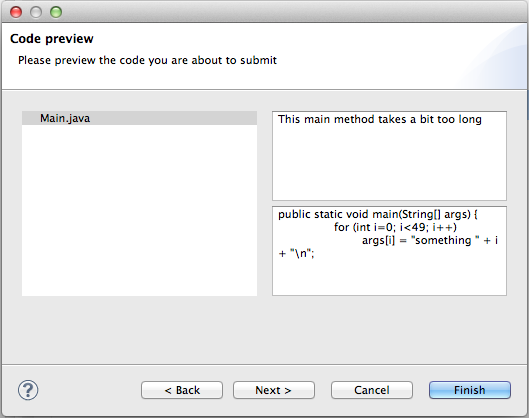
\includegraphics[width=\columnwidth]{wizard.png}
\caption{Adding comments for each snippet}
\label{fig:wizard}
\end{figure}

After entering all the details needed for a task, the user can then select the service to post it to. For the
moment we only offer integration with StackExchange, but other services can be added as well (like
oDesk, eLance etc). 

\section{Tying review outcomes to the code}

Once you submit the code, it can be difficult to remember what task relates to what code. In order to help
the programmer we decided to mark code snippets that were sent off for review. The icon on the right
rules notifies the developer if any replies have been received. 

\begin{figure}[hbt]
	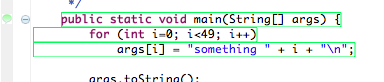
\includegraphics[width=\columnwidth]{marker.png}
\caption{The market that corresponds to the review}
\label{fig:marker}
\end{figure}

Figure~\ref{fig:marker} presents this concept. The code marked by the red box has been submitted of
review. Clicking on the marker will bring up the review task associated with it.

\section{Preliminary user study}
\section{Sketches}
\section{Conclusion}

\bibliographystyle{acm-sigchi}
\bibliography{paper}

\end{document}